\begin{figure}[h]
\centering
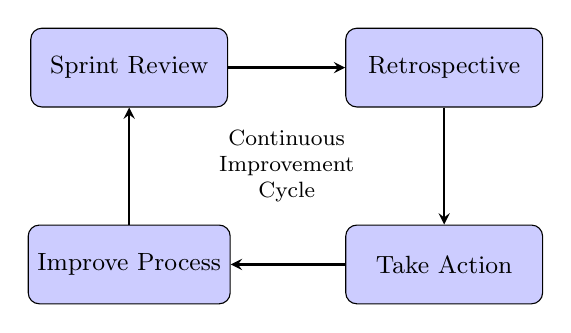
\begin{tikzpicture}
    % Define styles
    \tikzstyle{process} = [rectangle, rounded corners, minimum width=2.5cm, minimum height=1cm,
                          text centered, draw=black, fill=blue!20, font=\small]
    \tikzstyle{arrow} = [thick,->,>=stealth]

    % Nodes positioned absolutely
    \node[process] (review) at (0,0) {Sprint Review};
    \node[process] (retro) at (4,0) {Retrospective};
    \node[process] (action) at (4,-2.5) {Take Action};
    \node[process] (improve) at (0,-2.5) {Improve Process};

    % Arrows
    \draw[arrow] (review) -- (retro);
    \draw[arrow] (retro) -- (action);
    \draw[arrow] (action) -- (improve);
    \draw[arrow] (improve) -- (review);

    % Center label
    \node[font=\footnotesize, text width=2cm, align=center] at (2,-1.25) {Continuous\\Improvement\\Cycle};
\end{tikzpicture}
\caption{Continuous improvement cycle through regular sprint reviews and retrospectives}
\label{fig:improvement-cycle}
\end{figure}
